\section{Tercera pregunta de investigación}


\noindent\fbox{%
\parbox{\dimexpr\textwidth-2\fboxsep-2\fboxrule\relax}{%
\textbf{RQ3} ¿Como influye la variación de los parámetros de entrada a los algoritmos de análisis de relevancia y control de redundancia en los resultados de los modelos de clasificación?%
}%
}
\vspace{12pt}


\section{Estadísticas Descriptivas de FMeasure}

Las estadísticas descriptivas de la columna \textbf{FMeasure} son las siguientes:

\begin{itemize}
    \item Cantidad de registros (count): 13,916
    \item Media (mean): 0.547
    \item Desviación estándar (std): 0.104
    \item Valor mínimo (min): 0.274
    \item Percentil 25\%: 0.488
    \item Mediana (50\%): 0.529
    \item Percentil 75\%: 0.610
    \item Valor máximo (max): 0.844
\end{itemize}

Estos datos nos indican que la media de la medida F es aproximadamente 0.547, con una variabilidad moderada (desviación estándar de 0.104). El rango de los valores de FMeasure va desde 0.274 hasta 0.844.

\section{Correlación entre FMeasure, Rank y \(\beta\)}

A continuación, examinaré la correlación entre las columnas FMeasure, Rank y \(\beta\) para entender cómo se relacionan estas variables entre sí. Posteriormente, representaré visualmente estas relaciones.

\begin{figure}[H]
    \centering
    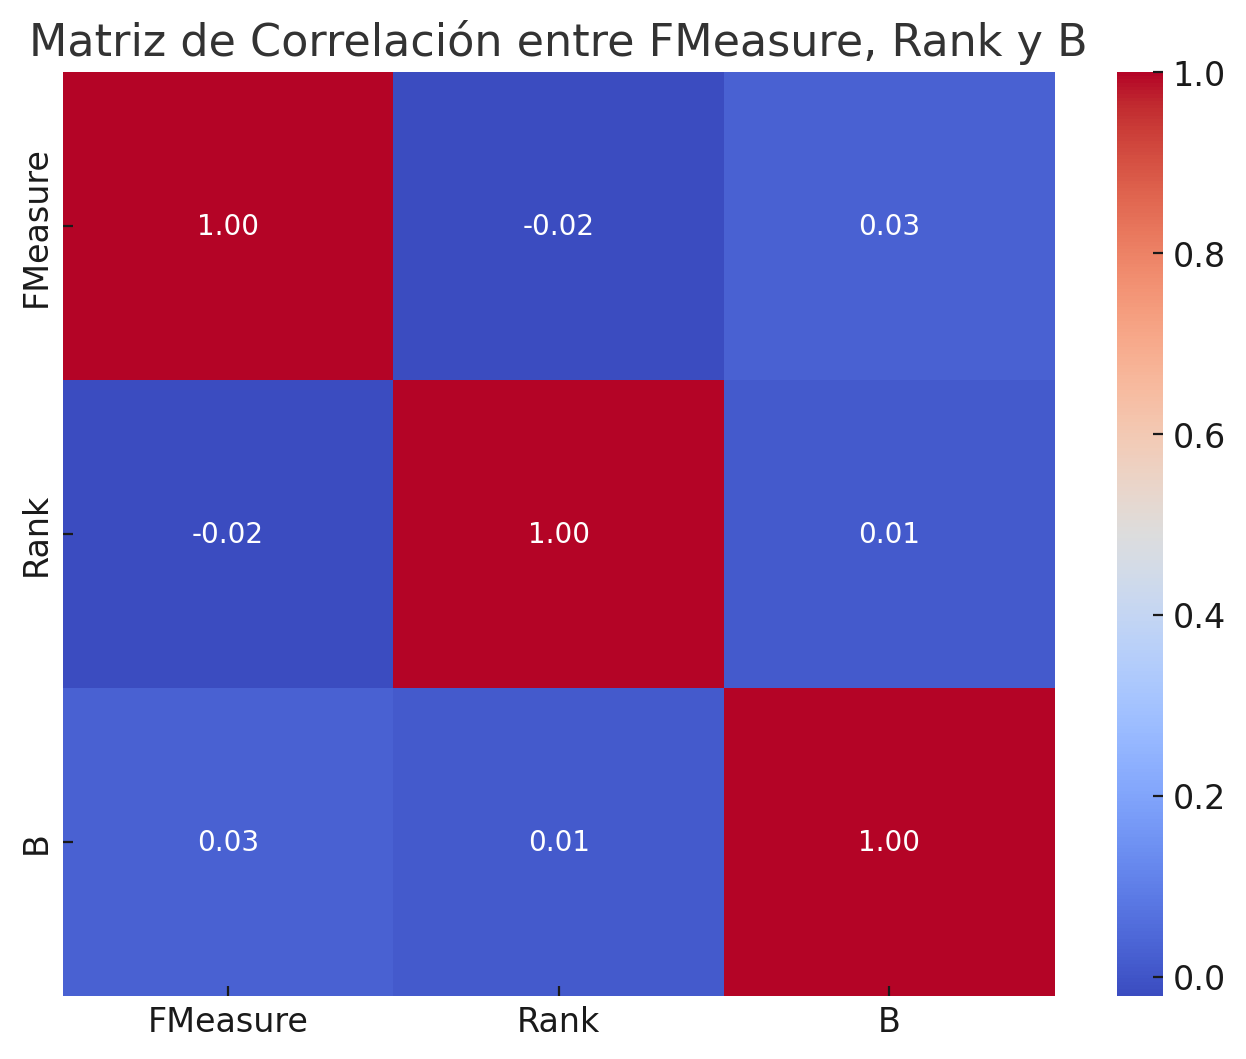
\includegraphics[width=100mm, height=80mm,]{chapters/chapter3/Sections/Research Questions/sections/RQ3/img/matriz.png}
    \setstretch{1} %Interlineado 1
	\captionsetup{labelsep=period, labelfont=bf}
    \caption{Frecuencia de cada métrica \(\beta\) y algoritmo de selección}
    \label{fig:frecuencyby}
\end{figure}

La matriz de correlación entre \textbf{FMeasure}, \textbf{Rank} y \textbf{B} revela lo siguiente:
{
\fontsize{14pt}{14pt}\selectfont
\begin{itemize}
    \item{Correlación entre FMeasure y Rank:} -0.021, lo que indica una correlación negativa muy débil. 
    \item{Correlación entre FMeasure y  \(\beta\):} 0.027, sugiriendo una correlación positiva muy débil. 
    \item{Correlación entre Rank y \(\beta\):} 0.011, lo que implica una correlación positiva casi inexistente.
\end{itemize}
}

Estas correlaciones sugieren que ni \textit{Rank} ni \textit{B} tienen una relación fuerte con \textit{FMeasure}.

Aunque no se observa una correlación fuerte entre los parámetros de entrada y el FMeasure, la Figura \ref{fig:FMeasure_rank_b} ilustra que, generalmente, valores menores de 'Rank' y mayores de 'B' se asocian con mejores resultados de FMeasure. Además, se identifica una tendencia descendente en los valores de FMeasure a medida que aumenta el 'Rank' para los tres valores distintos de 'B' evaluados.

\begin{figure}[H]
    \centering
    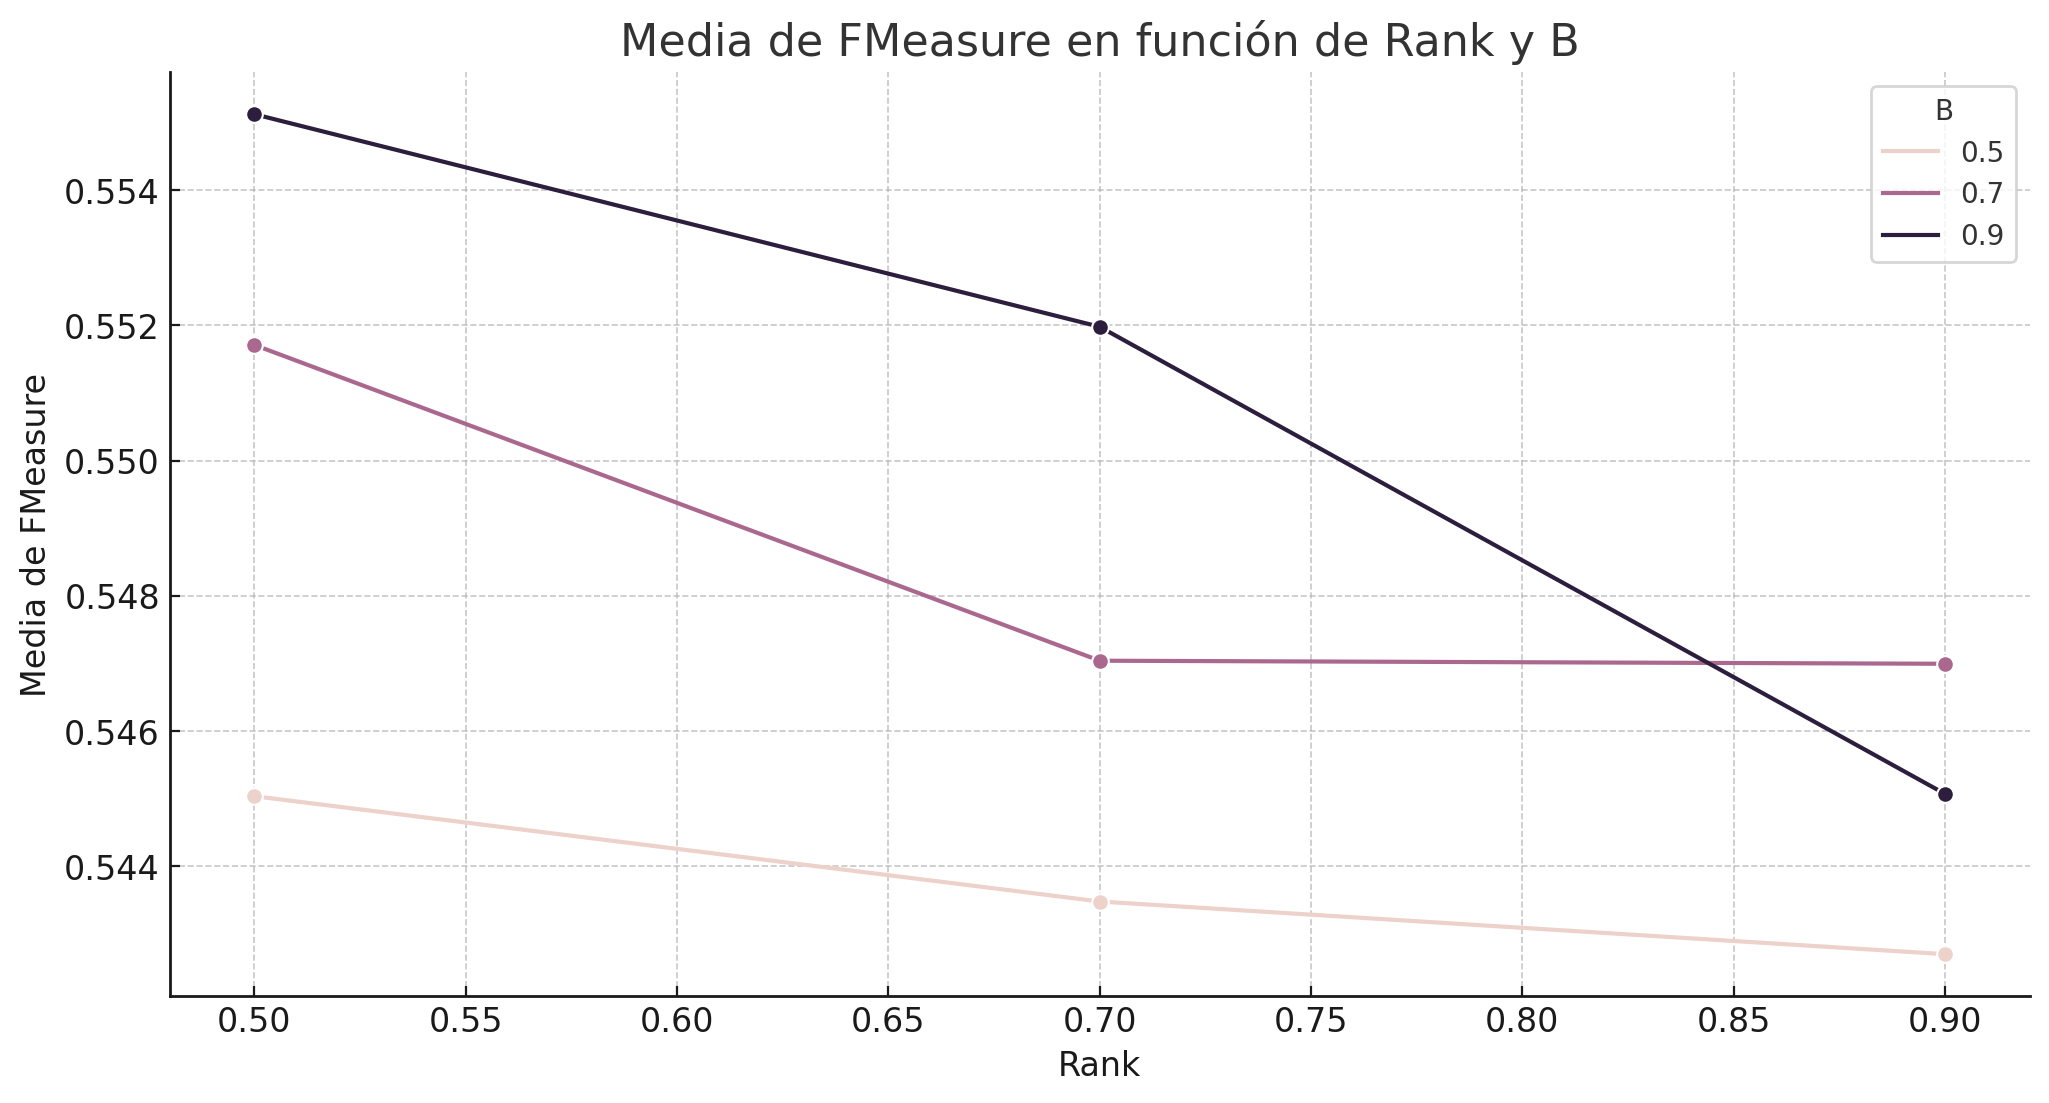
\includegraphics[width=150mm, height=120mm,]{chapters/chapter3/Sections/Research Questions/sections/RQ3/img/medida f en funcion de ran y b.png}
     \setstretch{1} %Interlineado 1
	\captionsetup{labelsep=period, labelfont=bf}
    \caption{Medición basada en rango y $\beta$}
    \label{fig:FMeasure_rank_b}
\end{figure}

En las tablas \ref{table:b_u_c_m}, \ref{table:b_u_c_c} y \ref{table:b_u_c_f} observamos que se obtienen valores similares a los obtenidos en la linea base (\ref{table:original_result_average}) pero con una disminución significativa de las características ingresadas en los modelos de clasificación. 

\noindent\fbox{%
\parbox{\dimexpr\textwidth-2\fboxsep-2\fboxrule\relax}{%
\textbf{Respuesta RQ3} 
En resumen, se observa que los parámetros de entrada utilizados en los algoritmos de análisis de relevancia y control de redundancia no presentan una correlación fuerte con el FMeasure. Sin embargo, se identifica que valores menores de 'Rank' y mayores de \( \beta \)  se asocian, en promedio, con mejores resultados de FMeasure. Paralelamente, se destaca que los algoritmos de selección reducen la cantidad de características ingresadas a los algoritmos, manteniendo o incluso mejorando los valores de FMeasure. Esto sugiere que, a pesar de la diversidad de los resultados, los valores seleccionados fueron eficaces para cumplir su propósito con un conjunto reducido de características.
}%
}
\vspace{12pt}